
\section{Agent Evaluation}\label{sec:evaluation_agent}
\begin{figure}
    \centering
    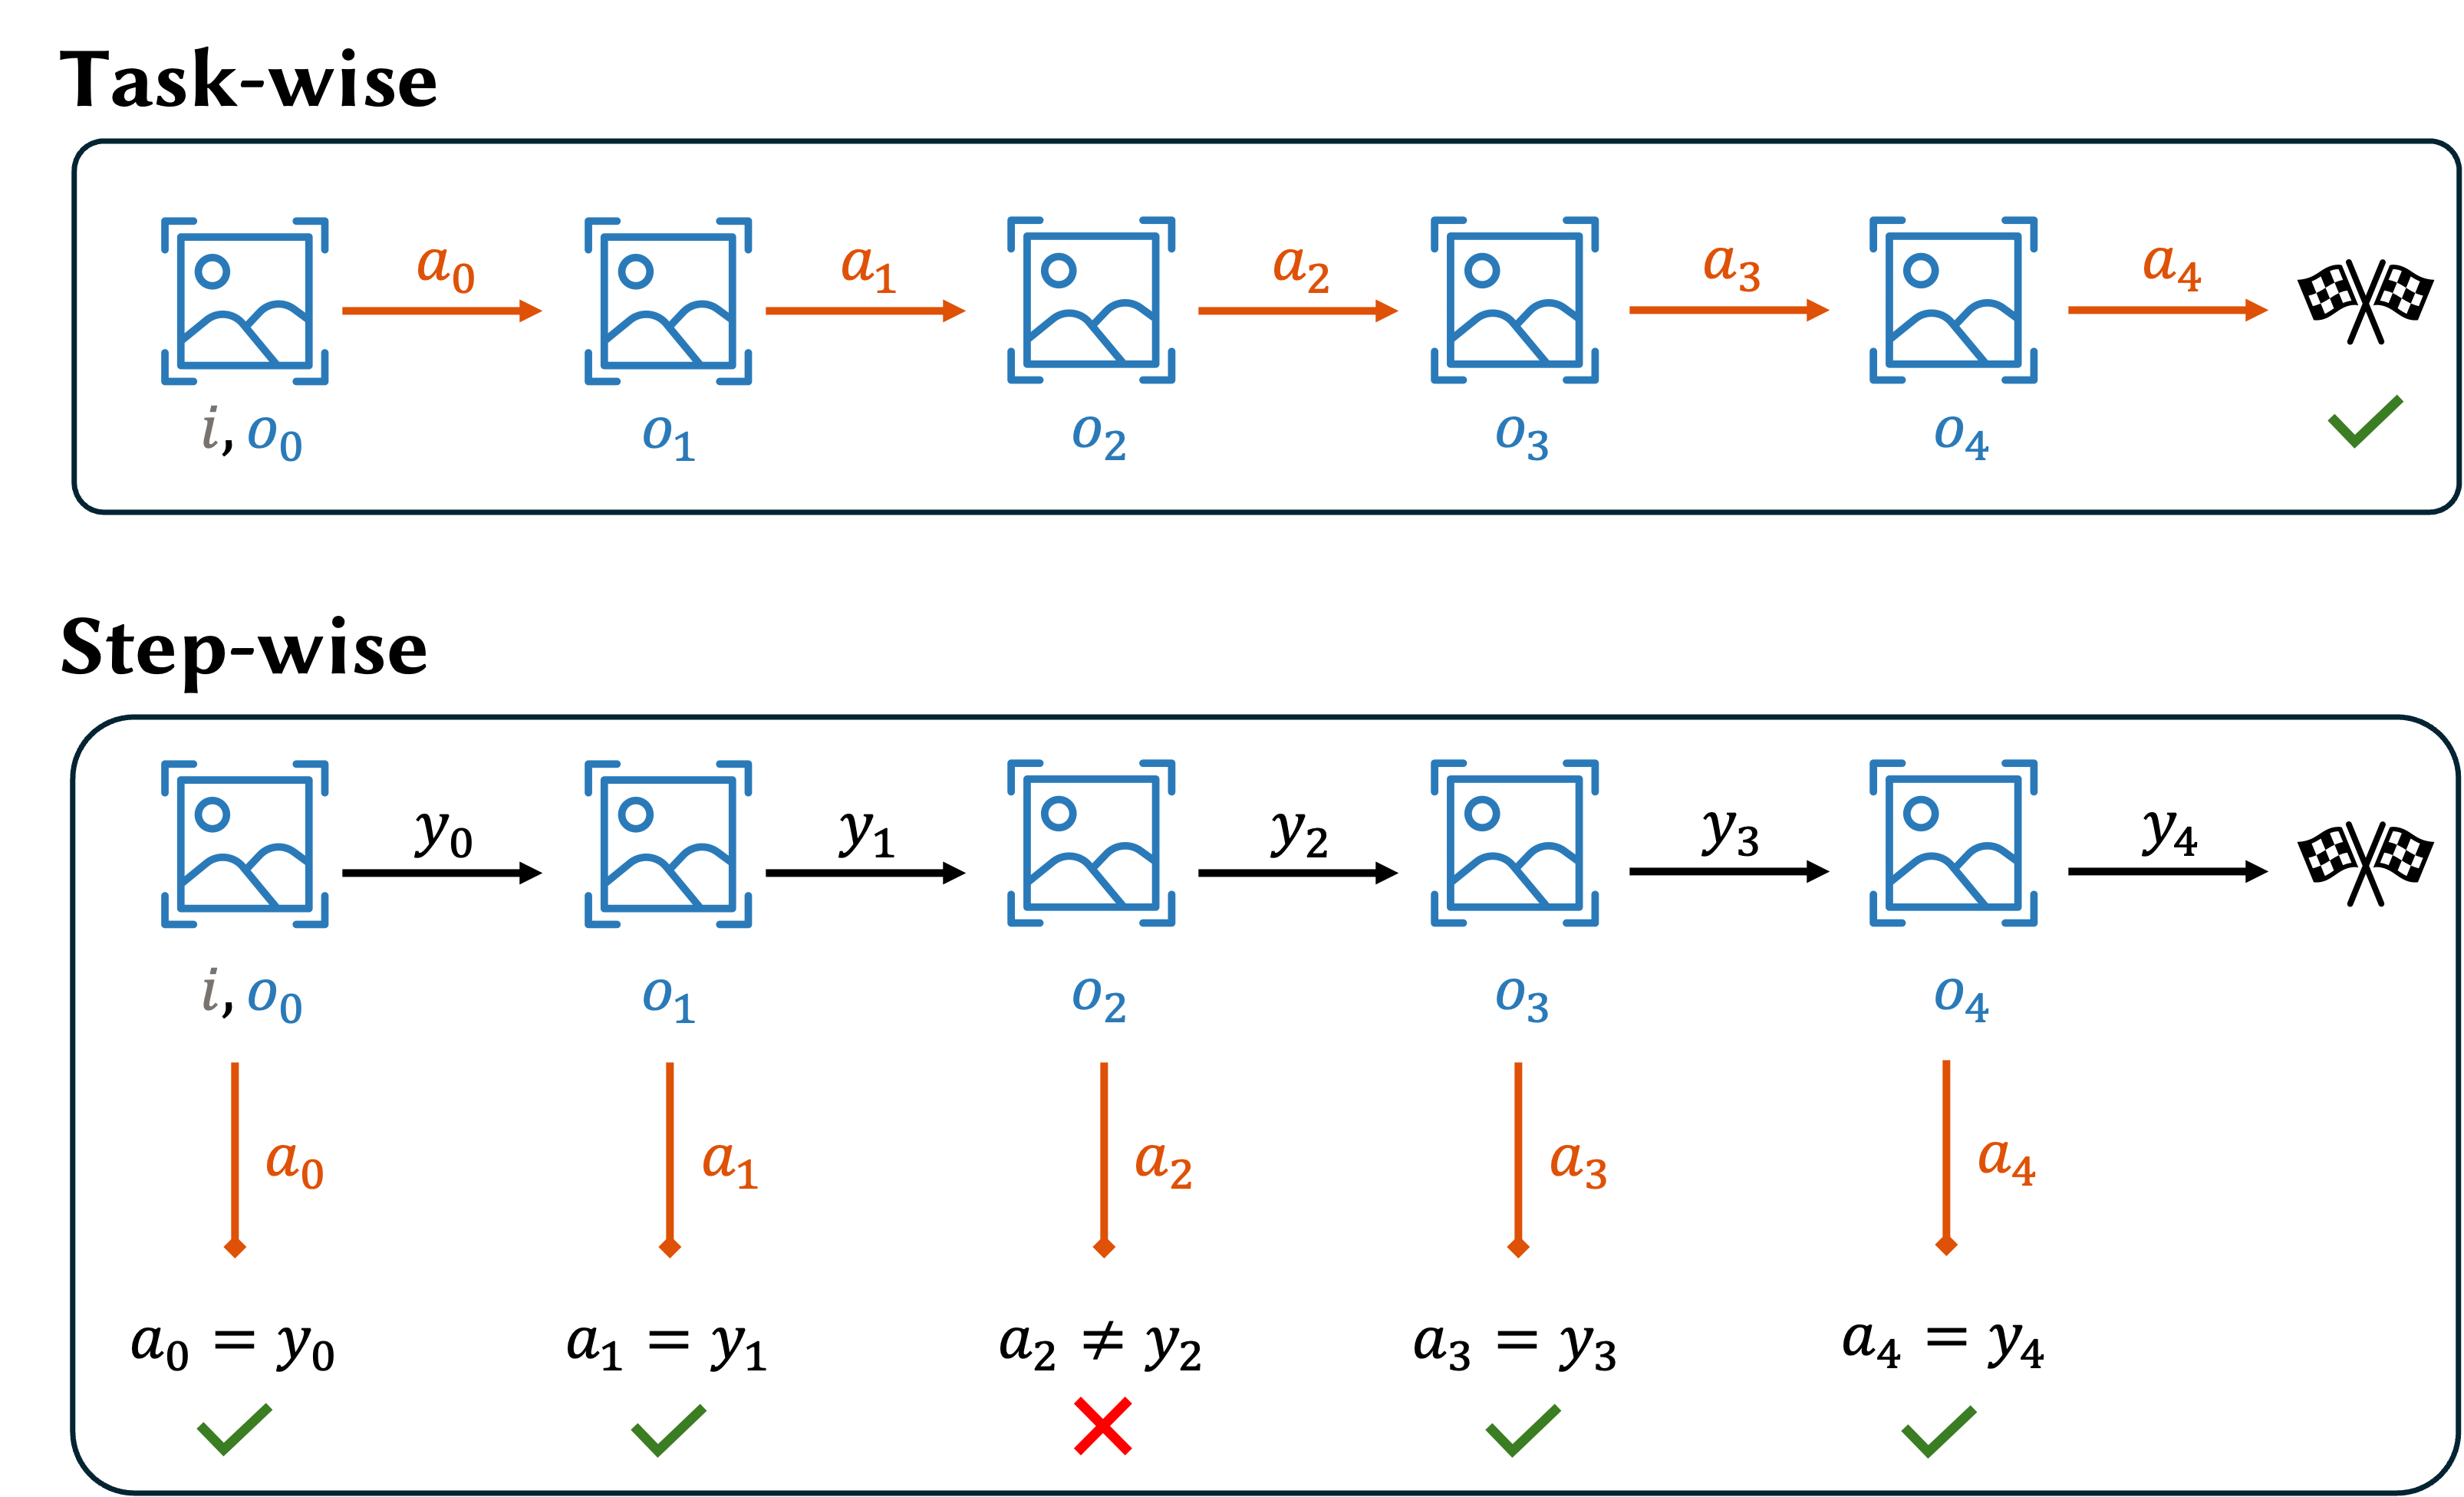
\includegraphics[width=0.6\linewidth]{figures/evaluation_types.png}
    \caption{Task-level metrics measure performance across individual tasks (instructions). Step-level metrics measure performance across individual steps (actions).}
    \Description{The figure contrasts two evaluation approaches. In both cases, a sequence of four generic observations and a single instruction is shown. In the task-wise evaluation (upper part), transitions between observations result from the model's predicted actions, and evaluation is performed only at the final observation. In the step-wise evaluation (lower part), transitions follow ground-truth actions, and the performance metric is computed after each individual prediction. A green checkmark visually indicates when evaluation occurs. Specific content of observations and instructions is not depicted, as they serve only to illustrate the evaluation paradigms.}
    \label{fig:evaluation_types}
\end{figure}

Various evaluation metrics are used in the current literature. 
We identify three groups of evaluation metrics (see also \cref{fig:evaluation_types}): \emph{Task-level metrics}, \emph{step-level metrics}, and \emph{other metrics}.  

\subsection{Task-Level Metrics}
Task-level metrics focus on the overall effectiveness of an agent in achieving an instruction $i$.
\emph{Task success rate} is the most common task-level metric, which measures the overall success rate of completing an entire task \citep{deng_mind2web_2023,zhang_android_2024}.
For controlled environments, the environment state indicates successful task completion. 
For offline datasets, an agent predicting the full trajectory correctly counts as successful task completion, termed \emph{offline task success rate} (also called complete match \citepeg{li_mapping_2020}).

The offline task success rate underestimates the actual task success rate, as it only considers a single recorded trajectory, whereas alternative valid trajectories may exist. Consequently, it serves as a \emph{lower bound} on the true task success rate.
To obtain a more accurate estimate, the \emph{online task success rate} can be used. To measure online task success rate, the agent must be deployed in its original environment, typically the live websites from which the offline dataset was collected. 
Human evaluators then determine whether the agent successfully completes the task \citep{zheng_gpt-4vision_2024, song_restgpt_2023, li_sugilite_2017}. Notably, \citet{zheng_gpt-4vision_2024} report that their agent's success rate increased from 12\% to 36\% when evaluated online, highlighting the limitations of relying solely on offline trajectories.
However, the reproducibility of the online task success rate poses a challenge, due to potential changes in the online environment and the potential for error in human evaluation \citep{reason1990human}.

Other, less common task-level metrics exist, often providing a more nuanced assessment of the agent's capabilities.
\emph{Task progress} measures the average task completion progress, meaning how far the agent, on average, is to complete a task \citepeg{sodhi_heap_2023, zhang_android_2024}.
\emph{Average reward} captures the average reward obtained across episodes within a controlled environment \citepeg{jia_dom-q-net_2019}. 
% It is worth noting that while these metrics are useful for comparing agents during development, they are not suitable for comparing agents across different environments, as they depend on the environment.

\subsection{Step-Level Metrics}

Step-level metrics focus on the overall effectiveness of an agent in predicting actions (steps) across tasks.
\emph{Step success rate} is the most common step-level metric, which assesses the accuracy of action prediction \citepeg{deng_mind2web_2023}.
In the literature, step success rate is also called \emph{partial match} \citepeg{li_mapping_2020} or \emph{action accuracy} \citepeg{wen_autodroid_2024}.

Each step (action) is part of a trajectory (a sequence of multiple actions), which in turn represents a single task in the dataset (comprising multiple tasks). Consequently, step-level metrics must define how to average step scores both within their trajectory and across tasks, similar to other fields like multi-class classification, where metrics are averaged within classes and across samples \citep{grandini2020metrics}.
Two natural approaches for averaging exist:

\begin{description}
    \item[Macro averaging:] 
        Step scores are averaged first within their respective trajectory and then across tasks. As a result, each step score is weighted by the inverse of its corresponding trajectory's length.
    \item[Micro averaging:] 
        Step scores are averaged across all steps (of all trajectories). This assigns equal weight to each step score regardless of trajectory length.
\end{description}

For computer use, \emph{macro averaging} seems to be the prevailing approach, established by Mind2Web \citep{deng_mind2web_2023} and adopted by subsequent work \citepeg{zheng_synapse_2024}.

Other less common step-level metrics include the \emph{action F1} score \citepeg{li_mug_2024}, \emph{action recall} \citepeg{li_glider_2021}, or measuring only if parts of the action are correct, like the \emph{element accuracy} for direct UI access actions \citepeg{deng_mind2web_2023}.
Finally, all step-level metrics only exist for offline datasets, as controlled environments' rewards do not indicate the correctness of individual actions.


\subsection{Other Metrics}

Other metrics in the literature measure performance indicators other than an agent's capabilities.
\citet{song_restgpt_2023} evaluate agent \emph{efficiency} by measuring the number of API calls required to execute an instruction successfully, emphasizing minimal resource usage during task execution.
\citet{zhang_ufo_2024} incorporate a safeguard mechanism to seek user confirmation before executing critical actions (e.g., delete) to build a safer and more trustworthy agent. The \emph{safeguard rate} measures how accurately the agent identifies sensitive actions and requests user confirmation. 

\subsection{Recommendations}
A standardized evaluation protocol is currently absent in the ACU literature. A key challenge lies in the prevalent use of custom datasets or modified benchmarks to highlight specific strengths \citepeg{wang_mobile-agent_2024,wen_autodroid_2024}, which limits comparability across studies.
For instance, in the MiniWoB++ benchmark \citep{shi_world_2017,liu_reinforcement_2018}, different studies have adopted varying subsets of tasks, complicating cross-study comparisons. \citet{humphreys_data-driven_2022} evaluated agents on all 104\footnote{MiniWoB++ currently includes 100 tasks, excluding four that violate the static assumption.} tasks, while \citet{zheng_synapse_2024} used 64 tasks and \citet{kim_language_2023} selected 55. 
Despite these differences between ACU evaluations, average task performance is compared directly, undermining fair assessment. 
For example, \citet[Figure 3]{zheng_synapse_2024} and \citet[Figure 4 (b)]{kim_language_2023} compared their average task performance on a subset of tasks with an ACU evaluated on the full benchmark.

Moreover, no consensus exists on how to measure agent performance.
Among the available performance metrics, the task success rate best reflects practical agent capabilities, as it evaluates whether an agent completes a task in its entirety.
In contrast, step-level metrics measure the performance across individual steps and can be misleading when assessing actual agent competence, as a single error in a lengthy action trajectory may have substantial real-world consequences but only a minor influence on step-level metrics.
Accordingly, we recommend that for evaluating performance, \textbf{ACU publications should report the task success rate as the primary metric on established and complete benchmarks}.

While task success rate can be reliably measured in controlled environments, it is challenging for offline datasets. 
Reporting the offline task success rate provides only a lower bound and might underestimate agent performance; reporting the online task success rate is labor-intensive and suffers from limited reproducibility due to evolving online environment conditions and different evaluation procedures.
In such offline dataset settings, the step success rate can serve as a reproducible proxy that must be interpreted with caution:
First, it is a conservative estimate of actual step correctness, as alternative valid actions are often not captured in the dataset and penalized as errors.
Second, higher step-level accuracy does not necessarily translate to higher task-level performance.

For evaluations on offline dataset benchmarks, we recommend reporting both the step success rate as a reproducible proxy metric and, where possible, the online task success rate as a measure of actual agent performance. To improve comprehensibility and traceability, the online evaluation protocol should be thoroughly documented, including details such as the date of the evaluation and any strategies used to mitigate human error \citep{reason1990human}.

Finally, ACUs must be capable of predicting a deliberate \texttt{stop} action to signal task completion. This capability is critical both for practical deployment and for correctly identifying when a task has been completed \citepeg{wang_mobile-agent_2024}. We therefore recommend requiring a \texttt{stop} action in ACU evaluations whenever feasible and suggest that future benchmarks enforce this requirement. For example, controlled environments could reward agents only after they reach the goal state and explicitly issue the stop action.
